\section{Evaluation}
\label{sec:evaluation}
This section presents a set of evaluations to show the performance of dynamic solution
compared with the original ingress controller. We establish a kubernetes cluster to be the base of the whole evaluation. Then we emulate five workload patterns and run them for twice, one with the original ingress controller equiped,
the other with our modified ingress controller equiped to compare their performance.
In summary, our results show that ....
with the original \gvirt{}. We run media transcoding and 2D/3D workloads in Linux, along with 2D/3D workloads in Windows.
We first compare the four reconstruction policies in \name{}, which confirms that  dynamic segmented partial reconstruction policy is with the best performance.
Then, we use this policy to compare \name{} with the original \gvirt{} as well as native performance.
In summary, our results show that \name{} achieves 85\% of native performance in most media transcoding test cases on Linux. For Linux 3D workloads, \name{} has
no negative effect in LightsMark, OpenArena, and UrbanTerror, respectively. For Linux 2D workloads, \name{} shows no negative effect in firefox-asteroids, firefox-scrolling,
midori-zoomed, and gnome-system-monitor, respectively. For windows 2D/3D workloads, \name{} has no negative effect on performance in 3Dmark06~{\cite{website:3dmark}},
Heaven3D~{\cite{website:heaven}}, and PassMark2D~{\cite{website:passmark}} respectively.

\subsection{Configuration}

Our evaluate platform consist of a tsung server, a original ingress controller, our modified ingress controller, several test applications and datebases.
All these are deployed as pods on kubernetes. Our kubernetes cluster is made up of a master and five nodes. The hardware configuration of master is Intel Core processor i7 6700 with 4 CPU cores(3.4Ghz), 64GB system memory and
a 1TB HDD disk. Nodes share the same configuration: Intel Xeon processor E5 2620 with 8 cores (2.10Ghz), 64GB system memory and a 1TB HDD disk. Many system components are deployed on the master, because it is responsible for managing the whole cluster, making it in high-load state, so we do not put any workload on master.
The tsung server is a request generator to emulate workload pattern for comparing performance, and we deploy it alone on node1 without putting any other application on node1 to make sure its perfomance on generating requests is not influenced by other unrelated factors during the evaluation.
Similarly, to gurantee the pure performance, we let ingress controller deployed alone on node2. The test application is a java web application connected to a database, it has several apis exposed, requests of different api have diverse consumption on CPU,memory,network and database.
The database is a MySQL instance accessed by the test applications. We deploy test applications and databases on node3, node4 and node5. With different strategies to generate workload, different number and placement of test application and database, we emulate fix workload pattern to
compare performance.

\subsection{Workload Pattern}
\label{subsec:workload_pattern}
In this section, we evaluate four workload patterns to evaluate performance of modified ingress controller compared with original ingress controller.
The workload patterns include initialization pattern, scaling pattern, node-blocking pattern and database-blocking pattern with four different setting of
endpoint placement, scaling strategies and workload composition.
\begin{figure}[!htb]
 \centering
 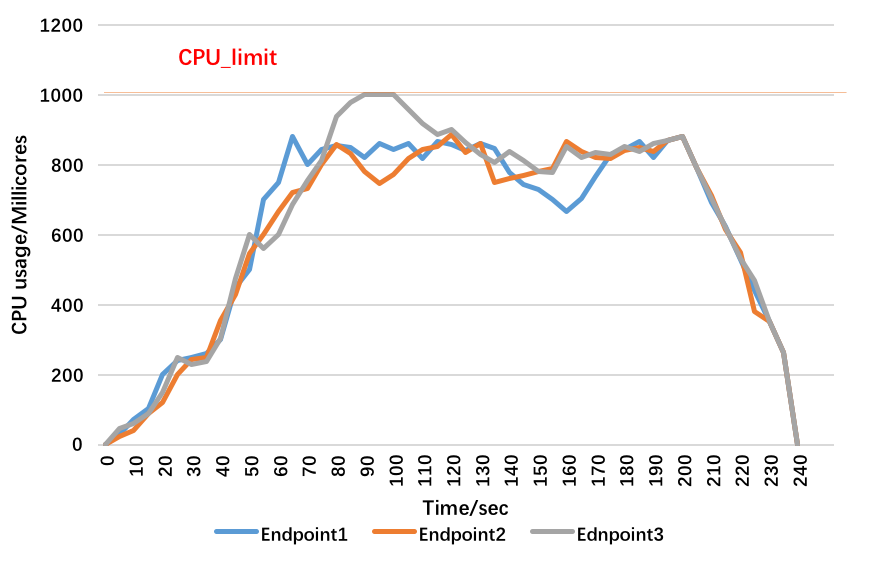
\includegraphics[width=0.45\textwidth]{images/data1.png}\\
 \caption{original controller under initialization pattern}
 \label{fig:original_initialization}
\end{figure}

\begin{figure}[!htb]
 \centering
 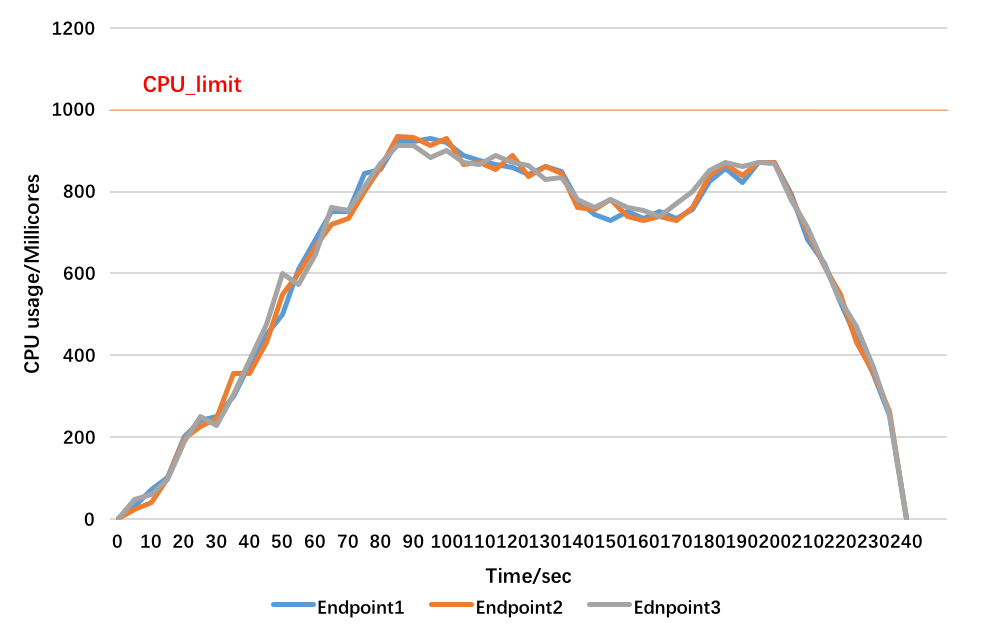
\includegraphics[width=0.45\textwidth]{images/data2.png}\\
 \caption{modified controller under initialization pattern}
 \label{fig:modified_initialization}
\end{figure}

Initialization pattern stands for the initial state when test applications are just deployed: we first deploy three replicas of test application, that is endpoint1 in node3, endpoint2 in node4 and endpoint3 in node5
to prevent that they are impacted by each other. After the deployment, we generate requests of all kinds at a fixed speed by tsung server to access test applications through ingress controller.
For convenience, we use the cpu statistics to present performance. Figure~\ref{fig:original_initialization} presents the performance of original ingress controller under initialization pattern and
figure~{\ref{fig:modified_initialization}} shows the performance of modified ingress controller. Result shows that for the original controller, load of endpoints become unstable and endpoint3 once becomes overhead(its cpu usage excceed its cpu limit) during 80s-100s, causing several
requests return 503 to tsung server, it confirms that the default round-robin algorithm only performs well when resource consumption of requests are almost the same, which is unpracticial. Figure~{\ref{fig:modified_initialization}} shows that
with the effort of modified ingress controller, there is no more overhead endpoint, load of endpoints are more even instead. More and more, table~{\ref{table:request_summary1}} points out that original ingress controller finishes 8892 reqeust, with 1108 503-requests, the
modified ingress controller finishes 10000 requests with no 503-request, and the total number of requests is 10000.
\hspace{0pt}
\begin{table}[htbp]
 \begin{center}
  \begin{tabular}{c|c|c|c}
   \hline
            & Finished & 503  & Total \\  \hline
   Original & 8892     & 1102 & 10000 \\ \hline
   Modified & 10000    & 0    & 10000 \\ \hline
  \end{tabular}
 \end{center}
 \caption{Request summary of initialization pattern}
 \label{table:request_summary1}
\end{table}


\begin{figure}[!htb]
 \centering
 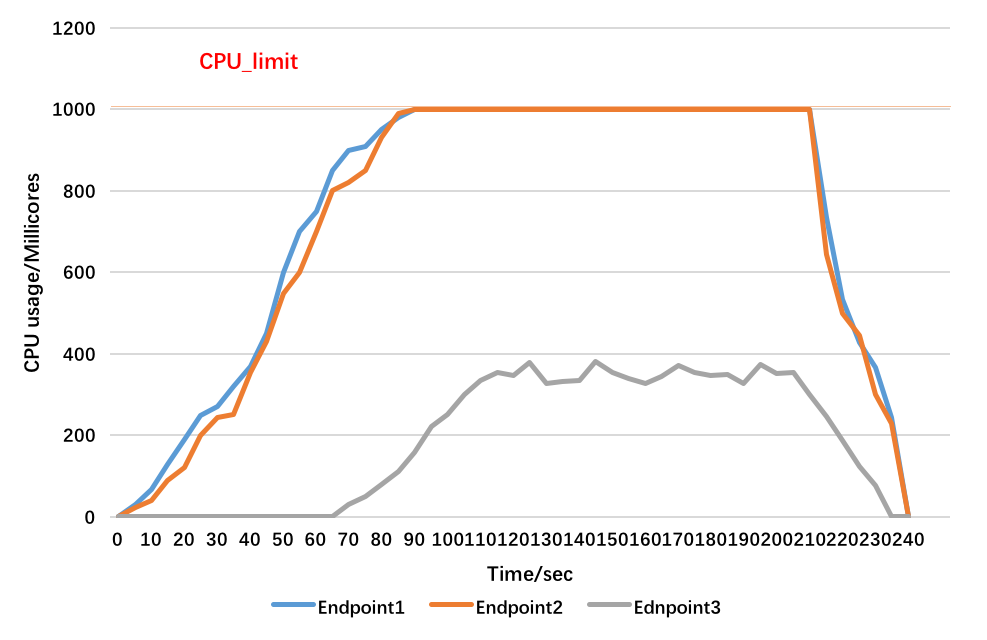
\includegraphics[width=0.45\textwidth]{images/data3.png}\\
 \caption{original controller under scaling pattern}
 \label{fig:original_scaling}
\end{figure}

\begin{figure}[!htb]
 \centering
 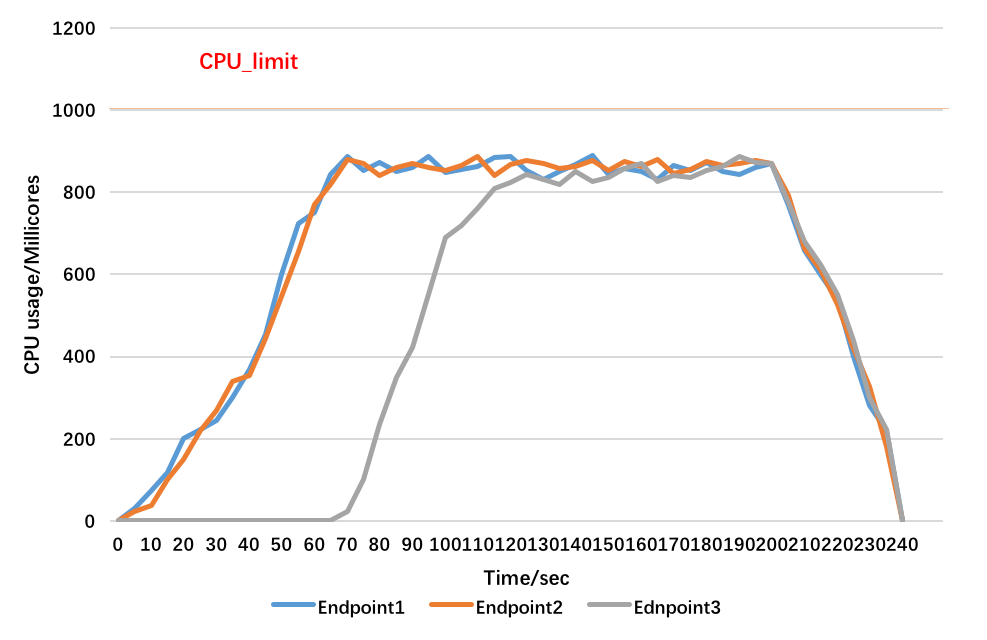
\includegraphics[width=0.45\textwidth]{images/data4.png}\\
 \caption{modified controller under scaling pattern}
 \label{fig:modified_scaling}
\end{figure}
Scaling pattern happens when administrator decides to scale up test applications because the workload is too large for current number of endpoint to handle.
To emulate this pattern, we first deploy endpoint1 in node3 and endpoint2 in node3 and generate high workload to keep these two endpoints in high-load state but not overload.
Then we deploy endpoint3 in node5 and increase the workload to the level that can keep three endpoints in high-load state ideally. Figure~{\ref{fig:original_scaling}} presents the performance of
original ingress controller under scaling pattern and figure~{\ref{fig:modified_scaling}} shows the performance of modified ingress controller. Result shows that that when we increse workload at 65s,
original ingress controller failes to dispatch appropriate workload to endpoint3, which should be assigned more workload to help endpoint1 and endpoint2. On the contrary,
the modified ingress controller succeeds to lead more workload to endpint3, as a result, no endpoint becomes overhead. Table~{\ref{table:request_summary2}} points out that original ingress finishes
xxx requests, with xxx 503-request while the modified ingress controller finishes xxx request with no 503-request, and the total number of reqeust is xxx.
\hspace{0pt}
\begin{table}[htbp]
 \begin{center}
  \begin{tabular}{c|c|c|c}
   \hline
            & Finished & 503  & Total \\  \hline
   Original & 5844     & 2956 & 8800  \\ \hline
   Modified & 8800     & 0    & 8800  \\ \hline
  \end{tabular}
 \end{center}
 \caption{Request summary of scaling pattern}
 \label{table:request_summary2}
\end{table}

Node-blocking pattern is established to evaluate performance of ingress controllers when their hosts are in high-load state. Firstly, we deploy endpoint1 in node3 and endpoint2 in node4.
Then we generate workload for node3 to keep it on high-load state, leaving only enough resource for endpoint1. After that, we generate high workload to keep these two endpoints in
high-load state but not overload and by comparing the RPS, we obtain performing disparity between original ingress controller and modified ingress controller. Through the comparison between
figure~{\ref{}} and figure~{\ref{}}, we find that it costs the original one about xxx second to handler xxx requests while it costs the modified one only YYY seconds, which demonstrates the fact
that load of host can affect the performance of endpoints. That is because the default isolation mechanism of 



\begin{figure}[!htb]
 \centering
 \includegraphics[width=0.45\textwidth]{figure/static.eps}\\
 \caption{\name{} with static reconstruction policy}
 \label{fig:static}
\end{figure}

We selectively switch 50, 100, 200, and 300 pages into the relaxed mechanism to evaluate the static partial reconstruction policy.
As shown in Figure~\ref{fig:static}, for cases without the issue static partial reconstruction policy achieves a worse performance than \gvirt{}.
The more pages that are switched into the relaxed mechanism, the worse the performance static partial reconstruction becomes.
For pages with few page table updates, reconstruction is meaningless. For cases with the Massive Update Issue, the static partial reconstruction
policy works and achieves a superior performance than \gvirt{}. Policy with 200 pages setting achieves the best performance for cases with the
Massive Update Issue, because policies with less pages cannot cover all the frequently accessed pages,
and policies with more pages include some useless pages.


\begin{figure}[htbp]
 \centering
 \includegraphics[width=0.45\textwidth]{figure/partial.eps}\\
 \caption{\name{} with dynamic partial reconstruction and dynamic segmented partial reconstruction}
 \label{fig:partial}
\end{figure}

Figure~\ref{fig:partial} confirms that the dynamic segmented partial reconstruction achieves better performance than dynamic partial reconstruction
comprehensively. \name{} performs better than \gvirt{} in issued cases, and has similar performance in normal cases.
The dynamic partial reconstruction switches the PTE pages into the relaxed mechanism progressively. However, some pages switched into the relaxed mechanism
may never be accessed again, and reconstructing these pages will produce extra overhead. Dynamic segmented partial reconstruction resets the relaxed pages,
after setting them to the guest pages. So for each cycle, dynamic segmented policy only reconstructs pages that need to be reconstructed.
Overall, dynamic segmented partial reconstruction is the most efficient policy, which is finally adopted by \name{}.

\subsection{2D and 3D performance}
In this section, we evaluate the 2D and 3D performance of \name{} under Linux and Windows. The results show
that \name{} has comparable performance with \gvirt{}'s 2D and 3D performance.
Moreover, \name{} achieves slightly superior performance than \gvirt{} in some cases.

\begin{figure}[htbp]
 \centering
 \includegraphics[width=0.45\textwidth]{figure/linux.eps}\\
 \caption{Performance running Linux 2D/3D workloads}
 \label{fig:linux}
\end{figure}

\begin{figure}[htbp]
 \centering
 \includegraphics[width=0.45\textwidth]{figure/windows.eps}\\
 \caption{Performance running Windows 2D/3D workloads}
 \label{fig:windows}
\end{figure}
\hspace{0pt}

Figure~{\ref{fig:linux}} demonstrates that \name{} achieves up to 94.63\% of native performance in 2D workloads and 88.81\% in 3D workloads on Linux.
Figure~{\ref{fig:windows}} demonstrates that \name{} achieves up to 88.81\% on Windows.

With the exception of the firefox-scrolling, urbanterror, warsow, SM2.0 and Pass2D, \name{} outperforms \gvirt{}. However,
the performance discrepancy between \name{} and \gvirt{} are acceptable.
